\documentclass{beamer}
\usetheme{metropolis}
\metroset{
    titleformat=regular,
    sectionpage=progressbar,
    numbering=none,
    background=light,
}
\usefonttheme[onlymath]{serif}

\setbeamertemplate{frametitle continuation}[from second]
\usepackage{import}
\subimport{./shared/}{preamble.tex}
%\subimport{./shared/}{project_definitions.tex}
\renewcommand\bibfont{\scriptsize}
\renewcommand{\bibsection}{}

\usepackage{appendixnumberbeamer}
\usepackage{booktabs}
\usepackage{caption}
\captionsetup[figure]{font=scriptsize}
\usepackage[scale=2]{ccicons}
\usepackage{csquotes}
\usepackage{dirtytalk}
%\usepackage[no-math]{fontspec}
%\setsansfont{Fira}
\usepackage{hyperref}
\usepackage{mdframed}
\usepackage{multicol}
\usepackage{setspace}
\usepackage{xspace}

\usepackage{amsmath}
\usepackage{amssymb}
\usepackage{empheq}
\usepackage{esint}
\usepackage{mathtools}
\mathtoolsset{showonlyrefs}

\usepackage{graphicx}
\graphicspath{ {images/} }
\usepackage{listings}
\usepackage{pdfpages}
\usepackage{pgfplots}
\usepgfplotslibrary{dateplot}

\newcommand{\fullPageImage}[1]{{
    \setbeamercolor{background canvas}{bg=black}
    \setbeamertemplate{navigation symbols}{}
    \begin{frame}[plain]
        \begin{tikzpicture}[remember picture,overlay]
            \node[at=(current page.center)] {
                \includegraphics[height=\paperheight]{#1}
            };
        \end{tikzpicture}
    \end{frame}
}}


\newcommand{\newsection}[1]{
  %\metroset{background=dark}
    \section{#1}
  %\metroset{background=light}
}

\newcommand{\pprime}{^{\prime}}
\newcommand{\sn}[2]{#1\times10^{#2}}
\newcommand{\snu}[6]{#1\times10^{#2}\,^{+\sn{#3}{#4}}_{-\sn{#5}{#6}}}
\newcommand{\snuwo}[3]{#1\,^{+#2}_{-#3}}
\newcommand{\unitsb}[1]{\,[\text{#1}]}
\newcommand{\functionof}[2]{#1\left(#2\right)}
\newcommand{\CPP}
{C\nolinebreak[4]\hspace{-.05em}\raisebox{.22ex}{\footnotesize\bf ++\,}}

\newcommand*\widefbox[1]{\fbox{\hspace{2em}#1\hspace{2em}}}
\newcommand{\Lagr}{\mathcal{L}}
\newcommand{\ham}{\mathcal{H}}
\newcommand{\infinitesum}[2]{\sum_{#1 = #2}^{\infty}}
\newcommand{\goodprime}{^{\prime}}
\newcommand{\tsi}[1]{\int_{\phi=0}^{2\pi}\int_{\theta=0}^{\pi}\int_{r=0}^{#1}}
\newcommand{\unit}[1]{\,\hat{\bm{#1}}}
\newcommand{\units}[1]{\,\text{#1}}
\newcommand{\vect}[1]{\mathbf{#1}}
\newcommand{\paren}[1]{\left(#1\right)}
\newcommand{\brackets}[1]{\left[#1\right]}
\newcommand{\abs}[1]{\left|#1\right|}
\newcommand{\anglers}[1]{\langle #1 \rangle}
\newcommand{\sinp}[1]{\sin{\paren{#1}}}
\newcommand{\cosp}[1]{\cos{\paren{#1}}}
\newcommand{\tanp}[1]{\tan{\paren{#1}}}
\newcommand{\expp}[1]{\exp\paren{#1}}
\newcommand{\thefrac}{\dfrac{n\pi}{d}}
\newcommand{\assolegendre}[1]{P_{#1}\paren{\cos{\theta}}}
\newcommand{\kg}{\units{kg}}

\newcommand{\partialwoa}[1]{\dfrac{\partial}{\partial #1}}
\newcommand{\partialtop}[2]{\dfrac{\partial#1}{\partial #2}}
\newcommand{\partiald}[2]{\dfrac{\partial}{\partial #2}\brackets{#1}}
\newcommand{\partialdd}[2]{\dfrac{\partial^2}{\partial^2 #2}\brackets{#1}}
\newcommand{\derivative}[2]{\dfrac{d #1}{d #2}}
\newcommand{\integral}[2]{\int_{#1}^{#2}}

\newcommand{\onec}{\frac{1}{\degree\text{C}}}
\newcommand{\degrees}[1]{\,\degree\units{#1}}
\newcommand{\cunits}{\,\frac{\units{J}}{\units{kg}\cdot\degrees{C}}}
\newcommand{\idcunits}{\,\frac{\units{J}}{\units{mol}\cdot\text{K}}}
\newcommand{\idc}{8.3145\,\frac{\units{J}}{\units{mol}\cdot\text{K}}}
\newcommand{\firstlTD}{the First Law of Thermodynamics}
% --------------------------------------------------------------------------- %
% Author Commands
% --------------------------------------------------------------------------- %
\newcommand{\theTitle}{\texttt{rkev}\\
{\small General Purpose $s$-stage Runge-Kutta and Evolutionary Optimizer}}
\newcommand{\theTitlecaps}{\MakeUppercase{\theTitle}}
\newcommand{\theAuthor}{Jackson L. Cole}
\newcommand{\theInstitution}{Middle Tennessee State University}

\newcommand{\projecturl}{\url{https://github.com/jacksonlanecole/rkev}}

%%%%%%%%%%%%%%%%%%%%%%%%%%%%%%%%%%%%%%%%%%%%%%%%%%%%%%%%%%%%%%%%%%%%%%%%%%%%%%%%
\title[\theTitle]
{\theTitle}
\subtitle{}
\author{\theAuthor}
\institute[MTSU]
{
    \theInstitution\\
    \medskip
    \texttt{me@jacksoncole.io}\enspace\textbullet\enspace\texttt{jacksoncole.io}
}
\date{Fall 2018}

% for a full page image
%\fullPageImage{path/to/image.ext}
%%%%%%%%%%%%%%%%%%%%%%%%%%%%%%%%%%%%%%%%%%%%%%%%%%%%%%%%%%%%%%%%%%%%%%%%%%%%%%%%
\begin{document}
\begin{frame}
    \titlepage
\end{frame}

\begin{frame}{What is a numerical integrator?}
    Let's say we are given a function describing the velocity of some object and
    an initial position.
    \begin{equation}
        \dot{x} = f\left(t, x\left(t\right)\right)
        \quad
        x\left(t_i\right) = x_i,
    \end{equation}
    If we are interested in the position, we can can approximate the solution
    to the ODE by using numerical integration.
    \begin{equation}
        \begin{aligned}
            x_{i+1} &= x_i + \int_{t_i}^{t_{i+1}}f(t, x(t))dt
            %= \boxed{\text{\scriptsize result of some numerical integration
            %method integrating } f\left(t, x(t)\right}}\\
        \end{aligned}
    \end{equation}
\end{frame}

\begin{frame}{The Workhorse: Fourth-order Runge-Kutta (RK4)}
\begin{minipage}{0.5\linewidth}
    \begin{itemize}
        \item Developed by Carl Runge and Wilhelm Kutta in early 1900s
        \item Most commonly used is the fourth-order Runge-Kutta (RK4)
    \end{itemize}
\end{minipage}%
\begin{minipage}{0.5\linewidth}
\begin{equation}
\small
\begin{aligned}
    k_1 &= \functionof{f}{t_i,\, x_i}\\
    k_2 &= \functionof{f}{t_i + \dfrac{1}{2}h,\, x_i + \dfrac{1}{2}k_1}\\
    k_3 &= \functionof{f}{t_i + \dfrac{1}{2}h,\, x_i + \dfrac{1}{2}k_2}\\
    k_4 &= \functionof{f}{       t_i + h,\,        x_i + k_3}\\
    x   &= x_i + \mathbf{\dfrac{1}{6}}\paren{k_1 + 2k_2 + 2k_3 + k_4}h\\
    t   &= t_i + h
\end{aligned}
\end{equation}
\end{minipage}


%Given a function $\functionof{f}{t, x}$, we
%can say that the derivatives are calculated as shown in equation \eqref{eqn:
%kderivatives}.
%\begin{equation}
%\begin{aligned}
%    k_1 &= \functionof{f}{t_i,\, x_i}\\
%    k_2 &= \functionof{f}{t_i + \dfrac{1}{2}h,\, x_i + \dfrac{1}{2}k_1}\\
%    k_3 &= \functionof{f}{t_i + \dfrac{1}{2}h,\, x_i + \dfrac{1}{2}k_2}\\
%    k_4 &= \functionof{f}{       t_i + h,\,        x_i + k_3}\\
%    \label{eqn: kderivatives}
%\end{aligned}
%\end{equation}
%The solution is updated
%\begin{equation}
%    x   = x_i + \mathbf{\dfrac{1}{6}}\paren{k_1 + 2k_2 + 2k_3 + k_4}h
%\end{equation}
%and the time is naturally updated by
%\begin{equation}
%    \label{eqn: time update}
%    t = t_i + h.
%\end{equation}
\end{frame}

\begin{frame}{RK4 Scheme: Equations}
    \small
\begin{equation}
\begin{aligned}
    % This is a bit too wide to adhere to 80 columns...
    k_1 &= f(t_i & + &(\mathbf{          0})h, &x_i& + & & (\mathbf{          0})k_1& + & (\mathbf{          0})k_2& + &           (\mathbf{0})k_3& + &           (\mathbf{0})k_4&)&\\
    k_2 &= f(t_i & + &(\mathbf{\frac{1}{2}})h, &x_i& + & & (\mathbf{\frac{1}{2}})k_1& + & (\mathbf{          0})k_2& + &           (\mathbf{0})k_3& + &           (\mathbf{0})k_4&)&\\
    k_3 &= f(t_i & + &(\mathbf{\frac{1}{2}})h, &x_i& + & & (\mathbf{          0})k_1& + & (\mathbf{\frac{1}{2}})k_2& + &           (\mathbf{0})k_3& + &           (\mathbf{0})k_4&)&\\
    k_4 &= f(t_i & + &(\mathbf{          1})h, &x_i& + & & (\mathbf{          0})k_1& + & (\mathbf{          0})k_2& + &           (\mathbf{1})k_3& + &           (\mathbf{0})k_4&)&\\
    x   &=       &   &                         &x_i& + &[& (\mathbf{\frac{1}{6}})k_1& + & (\mathbf{\frac{2}{6}})k_2& + & (\mathbf{\frac{2}{6}})k_3& + & (\mathbf{\frac{1}{6}})k_4 &]&h\\
    \label{eqn: more general rk4}
\end{aligned}
\end{equation}
\end{frame}

\begin{frame}{RK4 Scheme: Butcher Tableau}
\begin{figure}[h!]
    {\renewcommand\arraystretch{1.2}
    \begin{equation*}
        \begin{array}{ c|ccccc }
            0              & 0           & 0           & 0      &0\\
            \frac{1}{2}    & \frac{1}{2} & 0           & 0      &0\\
            \frac{1}{2}    & 0           & \frac{1}{2} & 0      &0\\
            1              & 0           & 0           & 1      &0\\
            \hline
            & \frac{1}{6} & \frac{1}{3}& \frac{1}{3}  & \frac{1}{6}\\
        \end{array}
    \end{equation*}
    \caption[Full Butcher Tableau for explicit fourth-order Runge-Kutta (RK4)] {
                Full Butcher Tableau for explicit fourth-order Runge-Kutta (RK4).
				This form comes from an abstraction of the full RK4 scheme.
            }
    \label{fig: full rk4 butcher}
    }
\end{figure}
\end{frame}

\begin{frame}{Butcher Tableaus and Runge-Kutta Geometry}
    \begin{minipage}{0.5\linewidth}
\begin{figure}[h!]
    \begin{equation*}
        \begin{array}{ c|ccccc }
            0      &        &        &        &\\
            c_2    & a_{21} &        &        &\\
            c_3    & a_{31} & a_{32} &        &\\
            \vdots & \vdots & \vdots & \ddots &\\
            c_s    & a_{s1} & a_{s2} & \dots  & a_{s,s-1} \\
            \hline
                   & b_{1}  & b_{2}  & \dots  & b_{s-1}   & b_{s}\\
        \end{array}
    \end{equation*}
    \caption[Butcher Tableau for explicit $s$-stage Runge-Kutta] {
                Butcher Tableau for explicit $s$-stage Runge-Kutta. This form of
                the tableau is found in many texts, so I will omit a reference
                here.
    }
    \label{fig:explicitbt}
\end{figure}
    \end{minipage}%
    \begin{minipage}{0.5\linewidth}
        \begin{figure}[h]
            \centering
            \frame{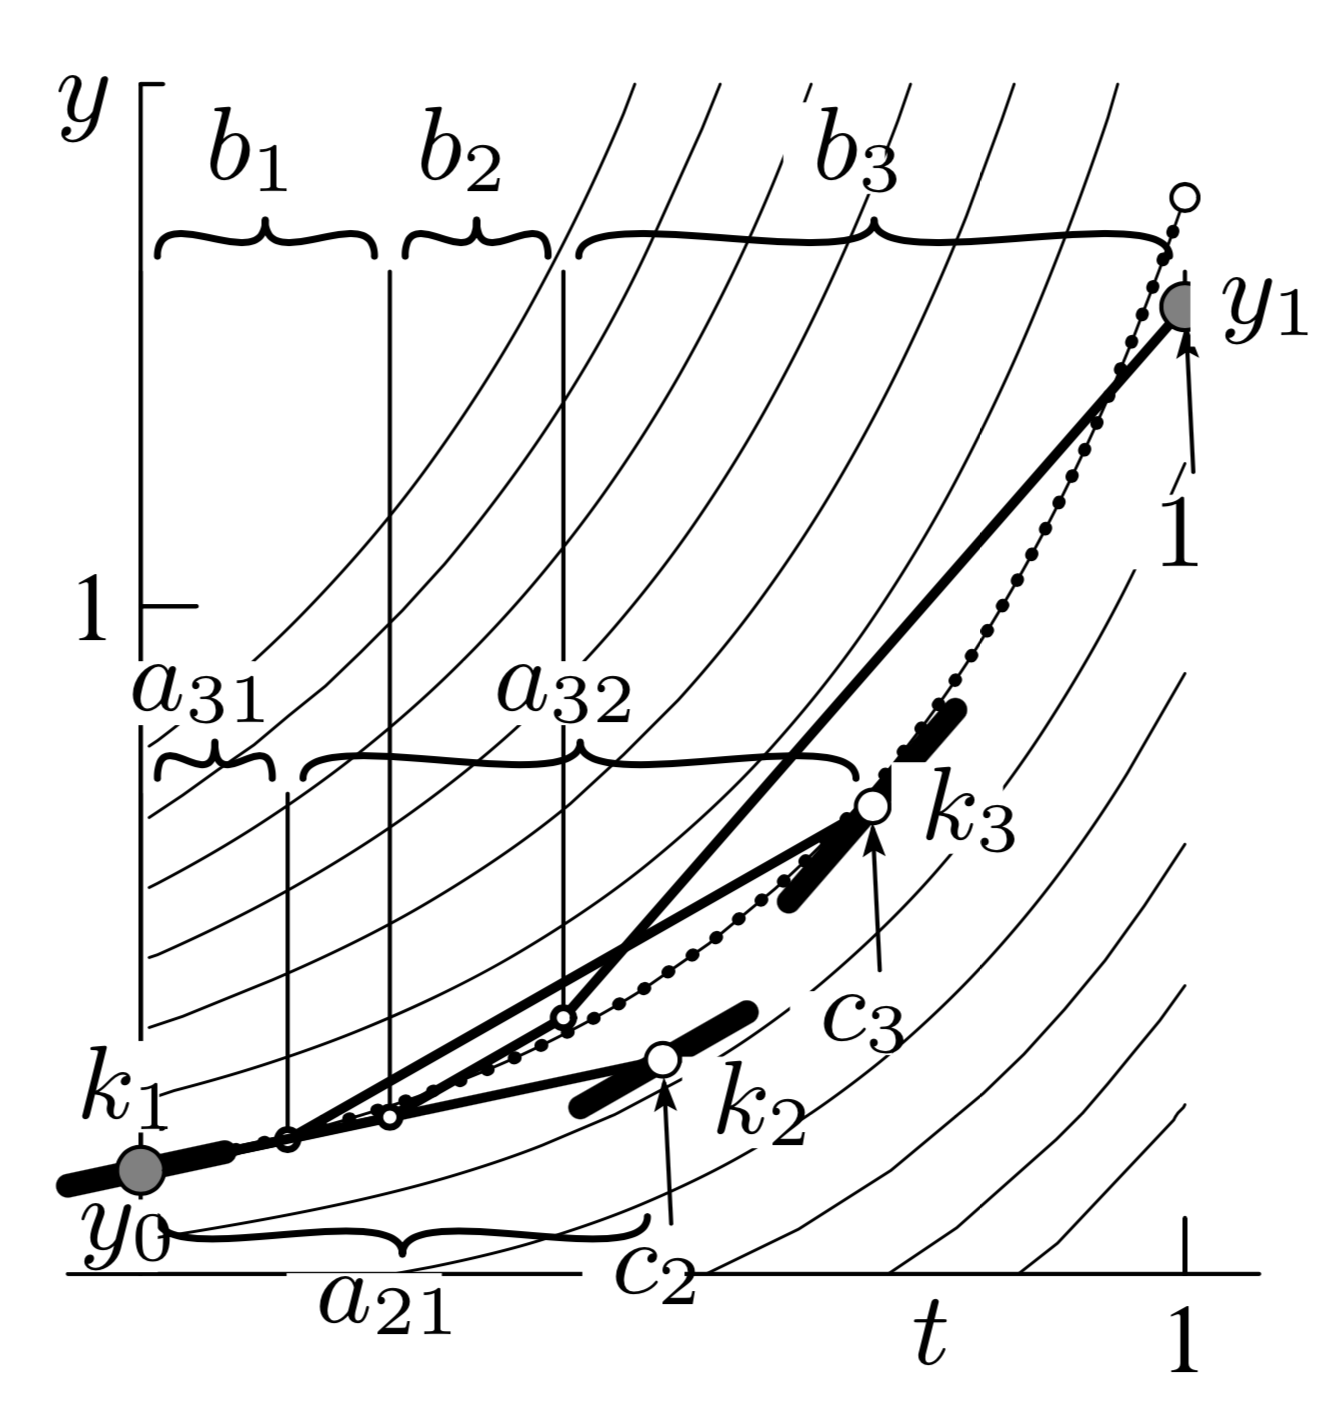
\includegraphics[width=0.9\linewidth]{images/rkdiagram.png}}
            \caption[Geometrical diagram of the Runge-Kutta method] {%
                Geometrical diagram of the Runge-Kutta method;
                The explicitly defined rows of Figure~\ref{fig:explicitbt} match
                with this diagram found in \citet{geometric_numeric}.
            }
            \label{fig:rkdiagram}
        \end{figure}
    \end{minipage}
\end{frame}


\begin{frame}{Specific Issues with Runge-Kutta in Astronomy}
    In the orbits of gravitationally bound systems, the total energy of the
    system should be conserved.

    Issue:
    \begin{itemize}
        \item Runge-Kutta methods do not preserve conserved quantities, and
            typically result in error that increases over long time integration.
        \item Essentially, RK methods integrate over a space in which a solution
            for the system can \textit{only} be approximated.
    \end{itemize}

    Solution:
    \begin{itemize}
        \item Symplectic integrators (preserve solution structure)
        \item \alert{Optimization of the Runge-Kutta scheme itself}
    \end{itemize}
\end{frame}

\begin{frame}{Goals and Benchmarks}
    Goals
    \begin{itemize}
        \item RK optimizer (i.e. Butcher Tableau optimizer)
        \item General-purpose RK Integrator
    \end{itemize}

    Benchmarks
    \begin{itemize}
        \item Energy error improvement in gravitational $n$-body simulations
    \end{itemize}
\end{frame}

\begin{frame}{General-purpose Runge-Kutta Integrator Specifications}
    Requirements:
    \begin{itemize}
        \item Must be able to perform \textit{any} RK
            integration scheme defined in a lower-triangular Butcher Tableau
        \item Must be callable in Python
        \item Must be able to call functions written in Python
    \end{itemize}
    If the appropriate initial conditions are defined, a standard fourth-order
    Runge-Kutta should be implemented as:
    \begin{figure}
        \begin{tikzpicture}
        \tikzset{font=\scriptsize}
            \node[io, text width=1.5cm](bt)
            {\tiny\arraycolsep=1.4pt\renewcommand\arraystretch{1.2}%
    \begin{equation*}
        \begin{array}{ c|ccccc }
            0              &             &             &        &\\
            \frac{1}{2}    & \frac{1}{2} &             &        &\\
            \frac{1}{2}    & 0           & \frac{1}{2} &        &\\
            1              & 0           & 0           & 1      &\\
            \hline
            & \frac{1}{6} & \frac{1}{3}& \frac{1}{3}  & \frac{1}{6}\\
        \end{array}
    \end{equation*}
            };
            \node[process, right = of bt, text width = 2cm] (rkintegrator)
            {%
                RK Integrator
            };

            \node[process, right = of rkintegrator, text width = 2cm] (result)
            {Result of RK4};

            \draw[arrow] (bt) -- (rkintegrator);
            \draw[arrow] (rkintegrator) -- (result);
        \end{tikzpicture}
    \end{figure}
\end{frame}

\begin{frame}{General-purpose Runge-Kutta Integrator Implementation}
    \begin{itemize}
        \item Written in C++
        \item Wrapped for Python using the Boost.Python library
        \item Accepts any lower-triangular square matrix
            \begin{itemize}
                \item i.e.\ this implementation can only handle \textbf{explicit}
                    Runge-Kutta schemes
            \end{itemize}
        \item Provides methods to run the full routine or step incrementally
        \item Provides methods to integrate a list of values (e.g.\ in an
            $n$-body simulation)
        \item Returns the result
    \end{itemize}
\end{frame}

\begin{frame}{\texttt{nbody} package}
    Born out of frustration with the overhead of $n$-body simulations of simple
    systems where randomizing masses is not feasible (i.e.\ specific two body
    systems)
    \begin{itemize}
        \item \texttt{Body} class
        \item \texttt{System} class
    \end{itemize}

    \alert{Reduces setup to initializing bodies, RKIntegrators, and calling the
    run method}
\end{frame}

\begin{frame}{$n$-body Simulation WITHOUT Energy Loss Correction}
        \begin{figure}[h]
        \centering
        \begin{minipage}{0.5\linewidth}
            \frame{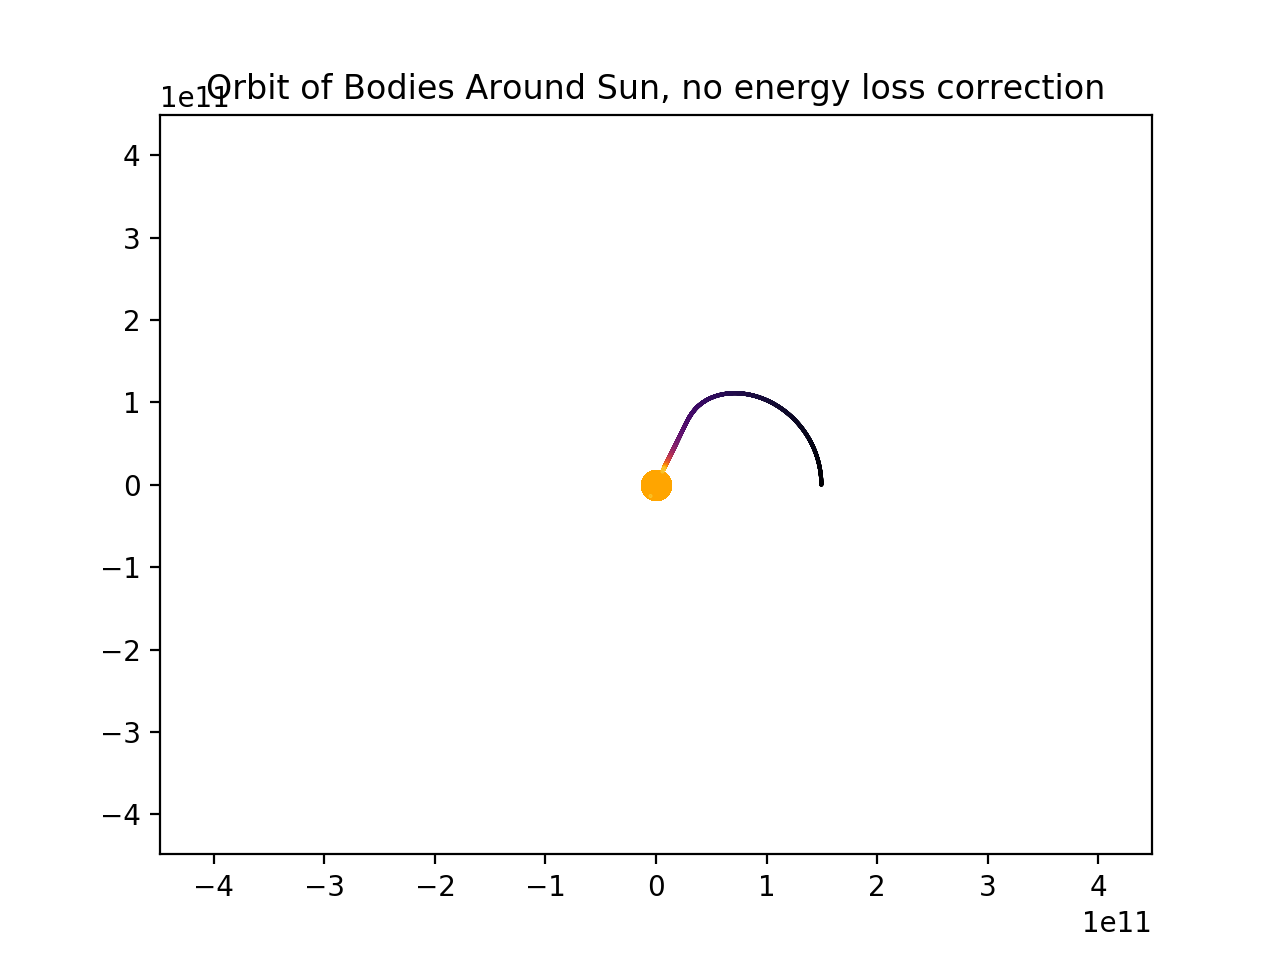
\includegraphics[width=\linewidth]{./images/decay2.png}}
        \end{minipage}%
        \begin{minipage}{0.5\linewidth}
            \frame{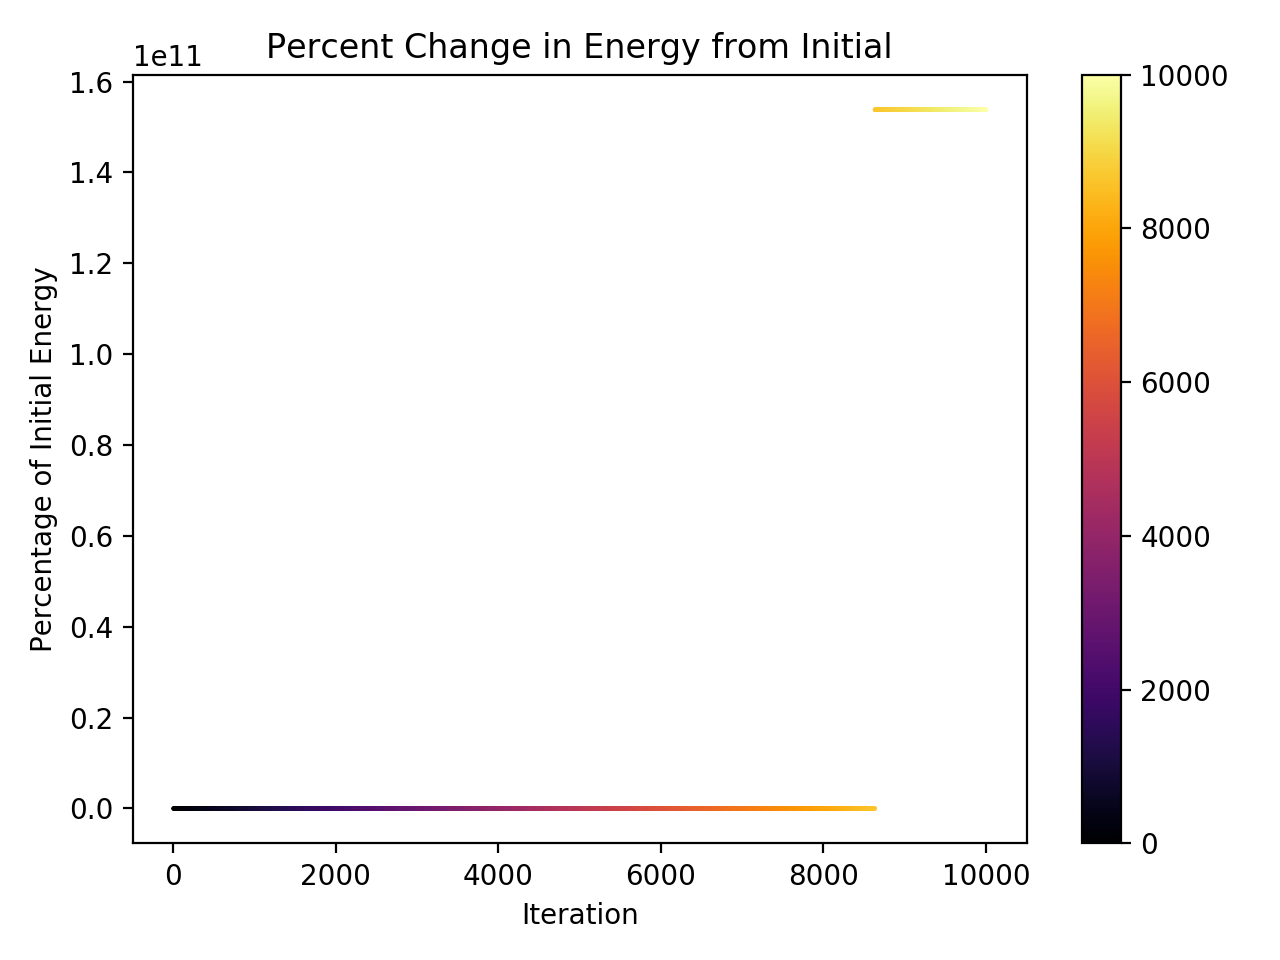
\includegraphics[width=\linewidth]{./images/energyerror2.png}}
        \end{minipage}%
        \caption{\textbf{LEFT:} Simulation of the Earth-Sun system showing heavy
        change in energy given the stability of the system. \textbf{RIGHT:}
            The change in energy of the system. The large \say{step} seen here
            could likely be improved by implementing adaptive step-size
            features in the RK Integrator.}
    \end{figure}
\end{frame}

\begin{frame}{Optimization with DEAP}
    DEAP $\to$ \textbf{D}istributed \textbf{E}volutionary \textbf{A}lgorithms in \textbf{P}ython
    \begin{itemize}
        \item Several generations of Butcher Tableaus are evaluated to minimize
            the \alert{change} in energy of the system
        \item The individual Butcher Tableaus are seeded from the more successful
            RK4 and RK38 methods (both developed by Runge-Kutta).
        \item The most successful individuals are crossed with a probability
            of 0.7.
    \end{itemize}
\end{frame}

\begin{frame}{$n$-body Simulation WITH Energy Loss Correction}
        \begin{figure}[h]
        \centering
        \begin{minipage}{0.5\linewidth}
            \frame{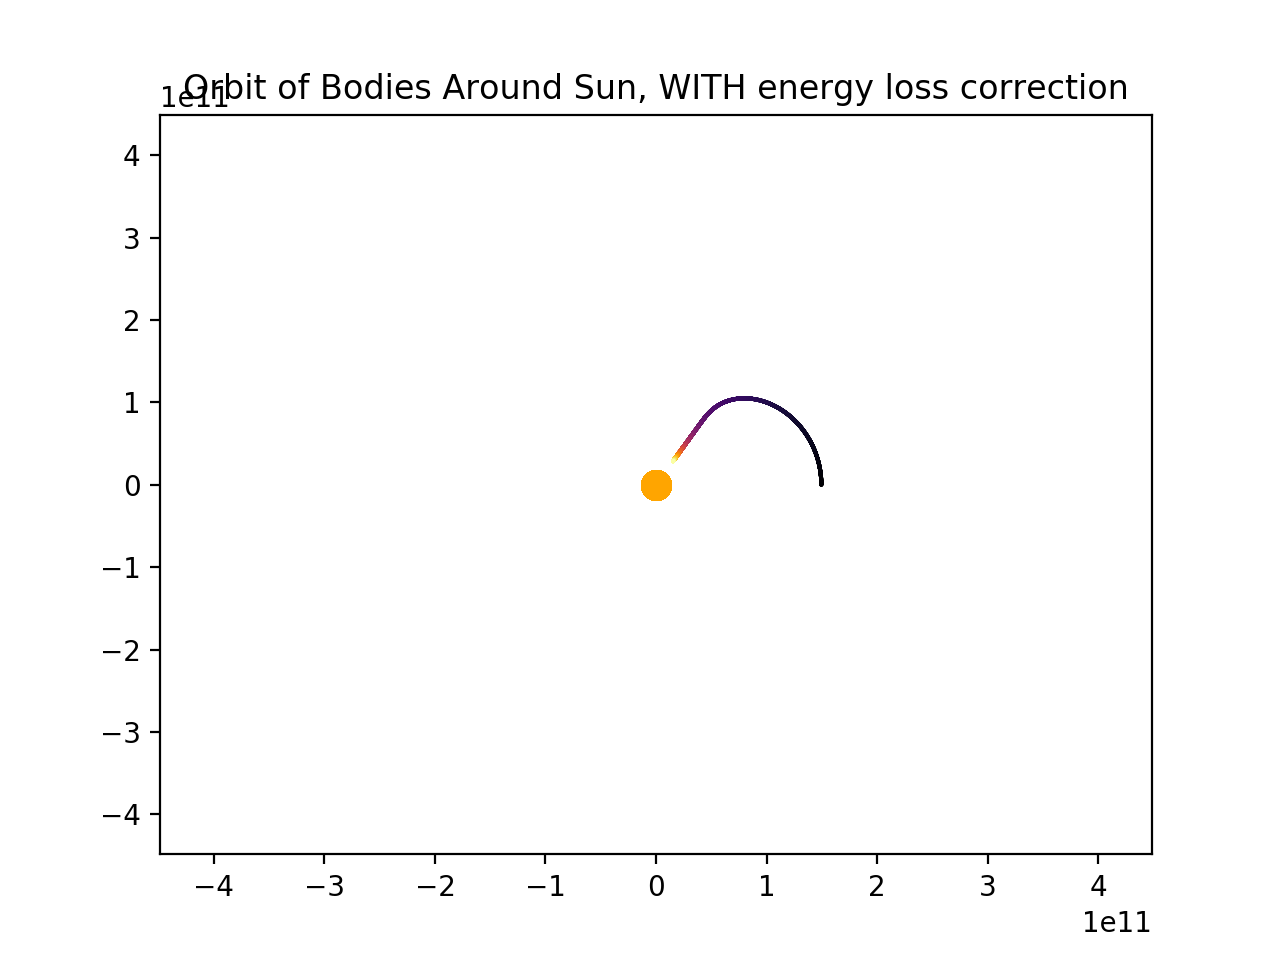
\includegraphics[width=\linewidth]{./images/decaycorrected.png}}
        \end{minipage}%
        \begin{minipage}{0.5\linewidth}
            \frame{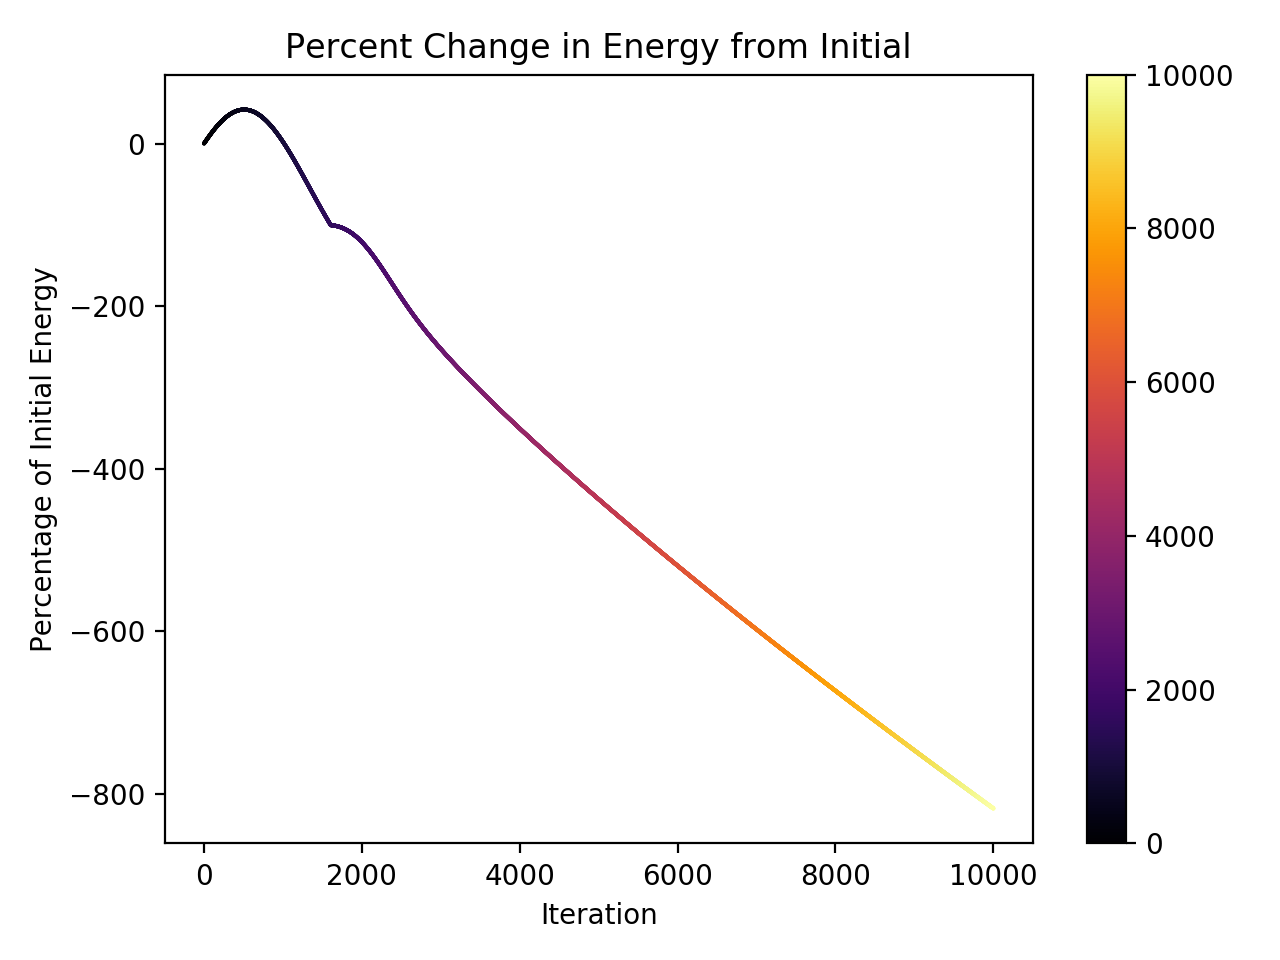
\includegraphics[width=\linewidth]{./images/energycorrected.png}}
        \end{minipage}%
        \caption{\textbf{LEFT:} Simulation of the Earth-Sun system still showing
        decay of the orbit, but the change can be really be seen in the energy
        plot.
        \textbf{RIGHT:}
            The change in energy of the system. This is significantly less of a
        change than the result of the prior integration.}
    \end{figure}
\end{frame}

\begin{frame}{Results, Conclusions}
    \begin{itemize}
        \item This method appears to have potential as a case-by-case optimizer
            for ODEs that have an associated cost function.
        \item Even with a standard RK4 method, a non-structure-preserving
            $n$-body code has been developed that is more intuitive and
            user-friendly.
    \end{itemize}
\end{frame}

\begin{frame}{Improvements}
    \begin{itemize}
        \item The results are, at most, promising. Although energy change is
            minimized, the resulting simulation still does not mirror the real
            system. Further work must be done to improve the $n$-body code
            \textit{and} the RK optimizer.
    \end{itemize}
\end{frame}

\begin{frame}[t,allowframebreaks]
    \frametitle{References}
    \bibliography{final}
\end{frame}

\end{document}
